\documentclass[border=6pt]{standalone}
\usepackage{tikz}
\usepackage[edges]{forest}
\usetikzlibrary{arrows.meta,positioning,calc,decorations.pathreplacing,shapes.geometric}
\begin{document}
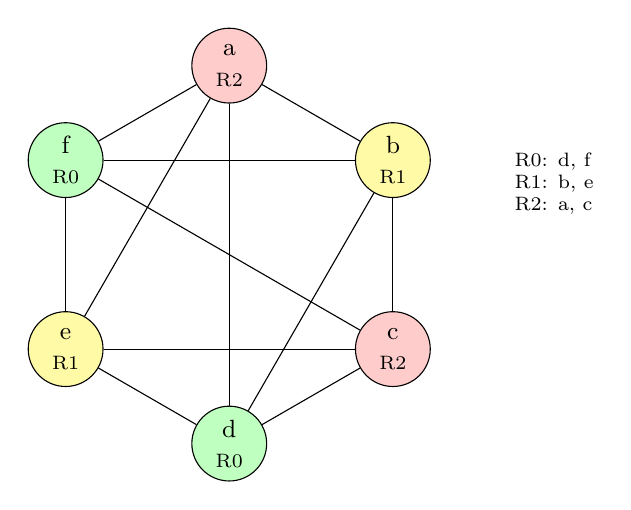
\begin{tikzpicture}[font=\small,v/.style={draw,circle,minimum size=0.95cm,inner sep=0pt,align=center}]
\node[v,fill=red!20] (a) at (0.000,2.400) {a\\{\scriptsize R2}};
\node[v,fill=yellow!35] (b) at (2.078,1.200) {b\\{\scriptsize R1}};
\node[v,fill=red!20] (c) at (2.078,-1.200) {c\\{\scriptsize R2}};
\node[v,fill=green!25] (d) at (0.000,-2.400) {d\\{\scriptsize R0}};
\node[v,fill=yellow!35] (e) at (-2.078,-1.200) {e\\{\scriptsize R1}};
\node[v,fill=green!25] (f) at (-2.078,1.200) {f\\{\scriptsize R0}};
\draw (a)--(b);
\draw (a)--(d);
\draw (a)--(e);
\draw (a)--(f);
\draw (b)--(c);
\draw (b)--(d);
\draw (b)--(f);
\draw (c)--(d);
\draw (c)--(e);
\draw (c)--(f);
\draw (d)--(e);
\draw (e)--(f);
\node[font=\scriptsize,anchor=west,align=left] at (3.5,0.9) {R0: d, f\\R1: b, e\\R2: a, c};
\end{tikzpicture}
\end{document}
